\documentclass{article}
\usepackage{amsmath}
\usepackage{bm}
\usepackage[capposition=top]{floatrow}
\usepackage{float}
\usepackage{amssymb}
\usepackage{amscd}
\usepackage{csquotes}
\usepackage{biblatex}
\addbibresource{bibliography.bib}

\usepackage{graphicx}
\graphicspath{ {./images/} }

\usepackage{amsthm}
\theoremstyle{definition}
\newtheorem{definition}{Definition}[section]
\newtheorem{theorem}{Theorem}[section]
\theoremstyle{definition}


\title{Knowledge Distillation in Matrix Product State Tensor Networks}
\author{Dereck Piché}
\date{\today}


\begin{document}
\maketitle

\section{Introduction}
Since the AlexNet\cite{alexnet} paper published in 2012, the use of artificial neural networks has gained a lot of popularity in several application areas. Because of their usefulness and generalisability, we would like to use them to train other models with radically different architectures. This is where knowledge distillation comes in. Suppose we have an already trained neural network that performs well on a certain task T. Then we can say that this neural network has knowledge about this task T. We would like to be able to transfer this knowledge from an already trained neural network into another system. This procedure is called \enquote{Knowledge Distillation}. This report is, foremost, an explanation of two particular MPS architectures, which we shall use as students. It also includes the results and analysis of several experiments were we distill knowledge of deep neural networks into MPS Tensor Networks.


\section{Knowledge Distillation}
Knowledge Distillation is a machine learning practice which involves
taking a trained model and using its parameters to train another one.
The already trained model is referred to as the \enquote{teacher}, and 
the model in which his "knowledge" is to be distilled is referred to as
the \enquote{student}. While this is a relatively novel technique, there are 
already several distinct approaches introduced by researchers.
In this project, we used two of these approaches. Our inspiration for the distillation 
methodology was found in a a 2021 survey which resumed the emerging 
practice \cite{Gou_2021}.

\subsection{Response-Based Knowledge Distillation}
The first approach we used was \emph{Response-Based Knowledge Distillation}. The idea of this approach is to stimulate the teacher and the student with some input and to try to minimise a certain loss function with respect to the teacher and student outputs. For classification tasks, it is recommended to use the Kullback-Leibler divergence as our loss function. 
\begin{equation}
    KL(P, Q) = \frac{1}{n} \sum_i^n Q \frac{log_e(Q)}{log_e(P)}
\end{equation}
Here, $Q$ is the distribution we are aiming for and $P$ is the one we have.

The reason is quite simple. Since it's a classification task, it is expected that the teacher and student will, given an input, return a probability distribution for each class. As is currently common, we used the softmax function on the logits of the student and the teacher in order to obtain probability distributions corresponding to the classes. 

\begin{equation}
    softmax(v_i) = \frac{e^{v_i}}{\sum_{j}{e^{v_j}}}
\end{equation}

Now, it would be logical to use a function aimed at measuring the difference between two probability distributions as our loss function. This is exactly what the Kullback-Leibler divergence is for.

\subsection{Layer-Based Knowledge Distillation}
Deep learning models work in layers of feature maps. It is hypothesized that
these different layers represent different layers of abstraction in the internal
representation of their input. If we use the Response-Based approach, it could prove difficult for gradient descent optimization to find these useful representation without a bit of help. {\it Layer-Based Knowledge Distillation} aims, as you might have guessed, aims to do precisely that. If our student model has some form of composition, we can train the parts separately. Thus, if an intermediate layer of the teacher $l$ were particularly useful, we could train a certain part of the student on the layer $l$ before proceding with the Response-Based approach.



\section{Tensor Networks}
Tensor Networks are mathematical objects which were created by physicists in order to help with the modelisation of quantum phenomena.
In 2017, researchers form the Flatiron institutes had the brilliant idea of using these networks as machine learning models \cite{stoudenmire2017supervised}. That is, to make them learn function in a supervised fashion. In order to make this report as self-contained as possible, we decided to provide an explanation of what they are. Some confusion can be avoided by mentionning that the expression \emph{Tensor Networks} refers, in the scientific community, to both a \emph{series of methods} and a \emph{notational system}.

\subsection{Tensors}
Before explaining the methods and the notational system, we shall disambiguate the meaning of the word \enquote{tensor}. In physics, tensors are often paired with transformation properties. 
However, in this report (and very often in the context of machine learning), we use the word \enquote{tensor} to refer to mathematical arrays of arbitrary dimensions denoted by indices. Here, the number of indices is called the \enquote{order} of the tensor, meaning that vectors are simply tensors of order $1$ and matrices tensors of order $2$. An exemple of a tensor of higher order would be $T_{i_1,i_2,i_3,i_4}$. This tensor is of order $4$.

\subsection{Contraction}
At the heart of tensor networks is the {\it contraction} operation.
Tensor Networks are used to compute a larger network by "contracting" several
smaller tensors over chosen indices. A "contraction" is simply an operation 
where we sum over indices. For example, the contraction of $A_{ijk}$ and 
$B_{ijk}$ on index $j$ will produce the tensor $C_{ik} = \sum_{j} A_{ijk} B_{ijk}$.
Evidently, the two indices present in a contraction must be of the same size.

\subsection{Tensor Networks as a graphical system of notation}
The main motivation behind the creation of Tensor Networks is to compute or approximate large tensors by {\it contracting} several smaller tensors over chosen indices. Our visual representation of tensors as a block of numbers stops at order $3$. 
This is all well and good until our conventional summation notation begins overclocking our poor brains. 
So, in order to make the manipulation of these network of tensors, mathematicians created a notational system. 
Tensors are represented as nodes where each vertex connected to the node represents one of the tensor's indices. 
If a vertex connects two nodes, it means that the indices shall be contracted in order to produce what we call, for lack of a better word, the \emph{post-contraction tensor}. 
It should be evident that by the definitions above, no node (tensor) is completely isolated in a tensor network, as it would be completely purposeless. 
The shape of the post-contraction tensor can be easily visually identified. we simply have to look for the vertices that are connected \emph{to a single tensor} in the network.
A simple tensor network can be found in figure \ref{fig:tensor_net}.
Let's translate this Tensor Network with the summation notation. First, we see that the result of the contractions of the smaller tensors $A$, $B$ and $C$ over their connected indices shall result in a tensor $T_{i, j, k}$, because $i$, $j$, and $k$ and the only indices that are not contracted. Since the other indices $l$, $m$ and $n$ are contracted, we will need to sum over them. Thus, the tensor represented in Figure \ref{fig:tensor_net} is equivalent to
\[ 
    T_{i, j, k} = \sum_{l, m, n} A_{j, l, m} B_{i, l, n} C_{m, n, k}
\]

\begin{figure}[hbt!]
    \centering
    \caption{A Very Simple Tensor Network Illustrating the notation.}
    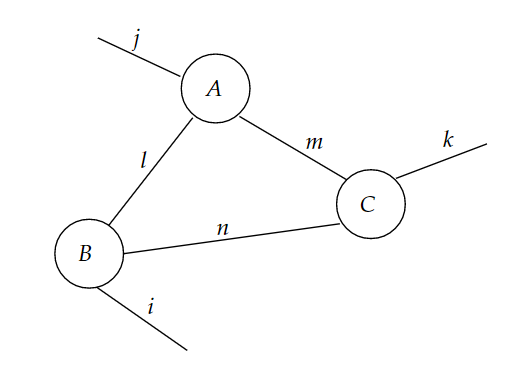
\includegraphics[width=0.8\textwidth]{images/2023-04-21-16-44-53.png}
    \label{fig:tensor_net}
\end{figure}

\subsection{Tensor Network Methods}
There are many ways of transforming a particular tensor into a tensor network. 
With time, some particular architectures became popular for their properties. These include the \emph{\it Matrix Product State (MPS)}, the \emph{Matrix Product Operator}, the \emph{MERA}, the \emph{Hierchical Tucker}, and much more.
Some are faster to compute, some are clearer, some are easier to train in a machine learning context, some are more visually appealing. One of these recurring architectures, the \emph{\it Matrix Product State (MPS)}, is at the core of this report.
Not only is there multiple valid ways of setting up the network for contractions, but there are also different ways to determine the order of contraction, since it has been shown that the order of contraction affects the computationnal complexity. It has even been shown that finding the optimal order of contraction is $NP-Hard$. All of these kinds of concepts are referred to by the expression \emph{Tensor Network Methods}. 

\section{Creating the Function we Shall Approximate}
In this report, we used the MPS tensor network to approximate a particular parameterizable function.
{\bf Troughout this report, the parameterizable function we are approximating with the MPS will be denoted by $\Upsilon_{T}$. }
We found it clearer to explain the $\Upsilon_{T}$ function we are approximating before introducing the MPS tensor network, as we we shall be able to explain the MPS through its use.
Now, enough talking (or rather, writing?), let's create the $\Upsilon_{T}$ function!

\subsection{Generating a Feature Space by Using the Kronecker Product}
Consider an input vector $\mathbf{x} \in \mathbb{R}^d$. Let $\phi : \mathbb{R} \to \mathbb{R}^{d_{\phi}}$ be a function which creates a feature map vector $\phi(x)$ from its input $x$.  We shall form the vector $\Phi(\mathbf{x})$ by taking the Kronecker product of the feature map $\phi$ of every element of the input vector $\mathbf{x}$.
\begin{equation}
    \Phi(\mathbf{x}) = \phi(x_1) \otimes  \phi(x_2) 
                \otimes (\dots) \phi(x_d)
\end{equation}
Here, the symbol $\otimes$ represents the Kronecker Product. The Kronecker Product is an extremely generalisable operation that can be applied to a pair of tensors of arbitrary order. However, we will limit our use of the Kronecker Product on tensors of order $1$, also called vectors. Here is a simple example that illustrates what the Kronecker Product does for simple vectors of integers.
\[
\begin{bmatrix}
    9 \\ 4
\end{bmatrix}
\otimes
\begin{bmatrix}
    6 \\ 8
\end{bmatrix}
\otimes
\begin{bmatrix}
    7 \\ 3
\end{bmatrix}
=
\begin{bmatrix}
    54 \\ 72 \\ 24 \\ 32
\end{bmatrix}
\otimes
\begin{bmatrix}
    7 \\ 3
\end{bmatrix}
=
\begin{bmatrix}
    378 \\ 162\\ 504 \\216\\ 168\\ 72\\ 224\\ 96
\end{bmatrix}
\]
As you can see, every element $i$ of the first operand vector becomes \emph{itself multiplied by the second operand vector}. Here's a slightly more abstract example which should clear things up:
\[
    \begin{bmatrix}
        v_1 \\ v_2
    \end{bmatrix}
    \otimes
    \begin{bmatrix}
        u_1 \\ u_2
    \end{bmatrix}
    =
    \begin{bmatrix}
        u_1 v_1 \\ u_2 v_1 \\ u_1v_2 \\ u_2v_2
    \end{bmatrix}
\]
Thus, if we perform a Kronecker Product on $n$ vectors, it will produce a vector such that every of its element is a multiplication of $n$ elements, each one from a different vector. We can thus interpret $\Phi(\mathbf{x})$ as being a feature space vector which \emph{captures the multiplicative interaction of the elements of the $\phi(x_i)$ feature vectors}. Here's a visual and intuitive way to think about the Kronecker Product applied to a set of vectors. Suppose we have the set of vectors and that we box an element of each one like so

\[
    \begin{bmatrix}
        \boxed{9} \\ 4
    \end{bmatrix},
    \begin{bmatrix}
        6 \\ \boxed{8} \\ 5
    \end{bmatrix},
    \begin{bmatrix}
        \boxed{7} \\ 3
    \end{bmatrix}
\]
Then the product of these elements,  $9\times8\times7=504$, will find itself in the vector $\bm{v}=
    \begin{bmatrix}
        9 \\ 4
    \end{bmatrix}
    \otimes
    \begin{bmatrix}
        6 \\ 8 \\ 5
    \end{bmatrix}
    \otimes
    \begin{bmatrix}
        7 \\ 3
    \end{bmatrix}
$. This statement would have been true had we chosen any other combination of the elements of each vector to box\footnote{Surround with a square.}. This is was what was meant when we said that the resulting vector captures the \emph{multiplicative interaction of the elements}.



\subsection{The multilinear feature map}
Now, which feature map $\phi$ shall we pick in order to define our particular $\Phi$?
For reasons which you will soon learn about, we picked the feature map
\begin{equation}
    \phi_{ml}(x) = 
    \begin{bmatrix}
        1 \\
        x
    \end{bmatrix}
\end{equation}
We call this particular feature map the \emph{multilinear feature map}, because, amazingly, when we use it, \emph{the elements of $\Phi(\mathbf{x})$ form a basis space of the multilinear functions on the elements of the vector $\mathbf{x}$}.
Understanding this statement without a bit of context and help is a tall order, so let's deconstruct it.
First, what is a multilinear function? A multilinear function is a multivariate function that is linear for every variable if all the other variables are considered as constants. For example, $f(x_1, x_2) = x_1 x_2 + 3$ is a multilinear function because the maps $x_1 \mapsto f(x_1, c) = x_1c  + 3$ and $x_2 \mapsto f(x_2, c) = x_2c  + 3$ are linear for any $c \in \mathbb{\mathbb{R}}$. However, $f(x_1, x_2) = x_1 x_2^2$ is not a multilinear function, because the map $x_2 \mapsto f(c, x_2) = c x_2^2$ is not linear for any $c \in \mathbb{R}$. A full explanation of vector spaces is out of the scope of this report. You can think of the space of multilinear function as a vector space. Without much rigour, we can say that this is the case because it is possible to describe any particular multilinear function by choosing the coefficients $c_i$ in this expression :
\begin{equation}\label{eq:basis}
    c_1 1 + c_2 x_1 + c_3 x_2 + c_4 x_3  + c_5 x_1 x_3 + c_6 x_1 x_2 + c_7 x_2 x_3 + c_8 x_1 x_2 x_3
\end{equation}
 example, if we want the function $f(x) = 3 + 4 x_2 x_3$, we simply need $c_1 = 3$, $c_7 = 4$ and the rest to be equal to $0$.

Let us show you explicitely what the Kronecker Product of the feature map $\phi_{ml}$ for the set of variables $\{x_1, x_2, x_3\}$
\[
    \Phi(\begin{bmatrix}x_1 \\ x_2 \\ x_3 \end{bmatrix})
    =
    \phi_{ml}(x_1) \otimes \phi_{ml}(x_2) \otimes \phi_{ml}(x_3)
    =
\]
\[
\begin{bmatrix}
    1 \\ x_1
\end{bmatrix}
\otimes
\begin{bmatrix}
    1 \\ x_2
\end{bmatrix}
\otimes
\begin{bmatrix}
    1 \\ x_3
\end{bmatrix}
=
\begin{bmatrix}
    1 \\ x_1
\end{bmatrix}
\otimes
\begin{bmatrix}
    1 \\ x_3 \\ x_2 \\ x_2 x_3
\end{bmatrix}
=
\begin{bmatrix}
    1 \\ x_3 \\ x_2 \\ x_2 x_3 \\ x_1 \\ x_1 x_3 \\ x_1 x_2 \\ x_1 x_2 x_3
\end{bmatrix}
\]
As, you can see, you can find every monomial found in expression \ref{eq:basis}.
Now, it should be clear that if we take the inner product of a vector $V$ and 
\[
    \langle V,  \Phi \left(\begin{bmatrix}x_1 \\ x_2 \\ x_3 \end{bmatrix}\right) \rangle
\]
which is equivalent to taking a linear combination of the elements of the vector, 
$\Phi(\begin{bmatrix}x_1 \\ x_2 \\ x_3 \end{bmatrix})$, we can express any multilinear function of the variables $x_1$, $x_2$ and $x_3$ by choosing the appropriate vector $V$.
\subsection{Linear Combinations}

At this point, you might be asking yourself, why go through all this? It has to do with expressivity. If we take the linear combinations of $\mathbf{x}$ directly, we will be limited to linear functions. However, in practice, many functions are fundamentally non-linear. They can't even be approximated well by linear functions. Thus, we project the initial vector $\mathbf{x}$ in a new non-linear space before applying the linear map. This is why we chose the $\phi_{ml}$. Multilinear functions are extremely expressive. Their limitations (as well as a way to bypass them) shall be discussed later in this report. \\ When we introduced $\Upsilon_{T}$, we said it was a parameterizable function. Thus, it is time to introduce the parameters. The parameters will be the coefficients of a linear map applied to the vector $\Phi(\mathbf{x})$.\\ 


As shown before before, if we apply a cross product to $\Phi(\mathbf{x})$, we obtain an extremely expressive function.
\[
    \langle
    \bm{v},
    \left(\phi_{ml}(x_1) \otimes \phi_{ml}(x_2)\otimes \dots \otimes \phi_{ml}(x_d) \right) \rangle
\]
where $\bm{v} \in \mathbb{R}^{2_d}$.
Now, here is the interesting part. Instead of doing this explicitely, we can reformulate the replicate the model by using a contraction between a tensor $T$ and the feature map vectors : 
\[
    \sum_{i_1, i_2, \dots, i_d} T_{i_1, i_2, \dots, i_d}
    \left(
    \begin{bmatrix}
        1 \\ x_1
    \end{bmatrix}_{i_1}
    \cdot
    \begin{bmatrix}
        1 \\ x_2
    \end{bmatrix}_{i_2}
    \cdot
    (\dots)
    \cdot
    \begin{bmatrix}
        1 \\ x_d
    \end{bmatrix}_{i_e}
    \right)
\]
This creates a fonction $f: \mathbb{R}^d \to \mathbb{R}$. If instead we want a function that maps to $\mathbb{R}^h$, we can add an index $h$ on the tensor $T$ such that it becomes $T^{h}_{i_1, i_2, \dots, i_d}$. At long last, we have all the ingredients to finally define the $\Upsilon_T :  \mathbb{R}^d \to \mathbb{R}^h$ function~:
\[
    \Upsilon_T(\mathbf{x}) =     \sum_{i_1, i_2, \dots, i_d} T^{h}_{i_1, i_2, \dots, i_d}
    \cdot
    \begin{bmatrix}
        1 \\ x_1
    \end{bmatrix}_{i_1}
    \cdot
    \begin{bmatrix}
        1 \\ x_2
    \end{bmatrix}_{i_2}
    \cdot
    (\dots)
    \cdot
    \begin{bmatrix}
        1 \\ x_d
    \end{bmatrix}_{i_d}
\]
You might be wondering why we didn't introduce the $Y_T$ function in this fashion right away. We simply thought that thinking about linear combinations of the elements given by the Kronecker Product gives a better intuition then the summation notation needed to describe the Tensor Network. Now, we have model that is, theoretically, trainable by the use of supervised learning. We simply have to modify the tensor $T$ according to our task, which represents the parameters of the model.

\section{The \emph{Matrix Product State} (MPS) Tensor Network}
The problem is that, as of now, the size of the tensor $T$ will grow exponentially with the number of dimensions of the input vector $\mathbf{x}$. Indeed, since our feature map $\phi_{ml}$ produces feature vectors of $2$ dimensions, the parameter tensor $T$ would have $h2^p$ parameters. For big inputs, it's more than we can handle. This is where the Tensor Network Methods come into play. We are going to approximate the tensor $T$ by using the \emph{Matrix Product State} Tensor Network in a creative way that was proposed in a previous paper \cite{stoudenmire2017supervised}.
\subsection{Building the model using a single MPS}
The MPS tensor network was created to approximate big tensors. It performs this by contracting multiple smaller tensors together.
\begin{equation} \label{eq:mps_approx}
T_{i_1, i_2, \dots, i_d} 
= 
\sum_{b_1,b_2,(\dots), b_d} t^{i_1}_{b_1} t^{i_2}_{b_1, b_2} t^{i_3}_{b_2 b_3} \dots  t^{i_d}_{ b_{d-1} } 
= \text{MPS approximation of $T$}
\end{equation}
In our case, the tensor we want to approximate has an extra index $h$. This index can be added to any tensor of the MPS. For example, we can put it in the third tensor of the chain :
\[
    \sum_{b_1,b_2,(\dots), b_d} t^{i_1}_{b_1} t^{i_2}_{b_1, b_2} t^{i_3, h}_{b_2 b_3} \dots  t^{i_d}_{ b_{d-1} } 
\]
As you can see, the original tensor $T$ is approximated by contracting the smaller tensors over the $b_i$ indices. The dimension of these indices is an hyperparameter of great importance. It is called the \emph{bond dimension} of the MPS. The higher the bond dimension, the closer we are to $T$. See \footnote{In a context of machine learning, it is also important to mention that the bigger the bond dimension, the bigger the expressivity of our model.}. To put it all together, we can approximate $\Upsilon_T(\mathbf{x})$ as such :
\[
    \Upsilon_T(\mathbf{x}) \approx
\]
\[
    \sum_{i_1, i_2, \dots, i_d}
    \left(
    \sum_{b_1,b_2,(\dots), b_d} t^{i_1}_{b_1} t^{i_2}_{b_1, b_2} t^{i_3, h}_{b_2 b_3} \dots  t^{i_d}_{ b_{d-1} } 
    \right)
    \cdot
    \begin{bmatrix}
        1 \\ x_1
    \end{bmatrix}_{i_1}
    \cdot
    \begin{bmatrix}
        1 \\ x_2
    \end{bmatrix}_{i_2}
    \cdot
    (\dots)
    \cdot
    \begin{bmatrix}
        1 \\ x_d
    \end{bmatrix}_{i_d}
\]
We can use the Tensor Network Notation in order to visualise the process and to make things clearer. The $\Upsilon_T$ function can be visualised in Figure \ref{fig:full_tensor_model} and it's approximation $\Upsilon_{MPS}$ can be visualised in Figure \ref{fig:mps_tensor_model}.
\begin{figure}[hbt!]
    \centering
    \caption{The $\Upsilon_T$ function visualised with the Tensor Network Notation.}
    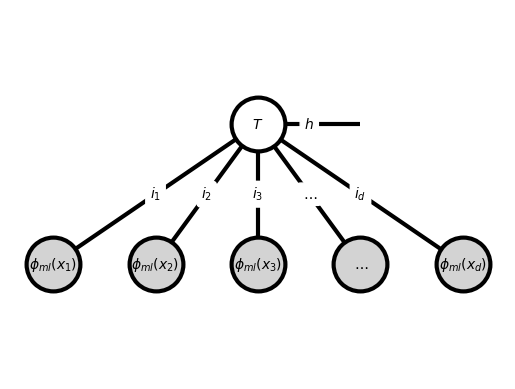
\includegraphics[width=0.7\textwidth]{images/2023-04-20-11-02-45.png}
    \label{fig:full_tensor_model}
\end{figure}

\begin{figure}[hbt!]
    \centering
    \caption{The $\Upsilon_{MPS}$ function visualised with the Tensor Network Notation.}
    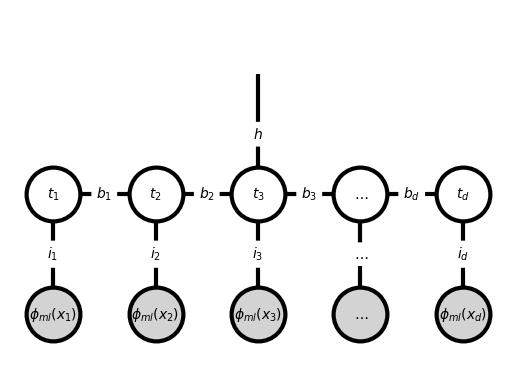
\includegraphics[width=0.7\textwidth]{images/2023-04-20-12-41-57.png}
    \label{fig:mps_tensor_model}
\end{figure}

\subsection{Composition of MPS}
As mentionned before, taking a linear map of the Kronecker Product applied to a set of the local feature map 
$ x \mapsto \begin{bmatrix} 1 \\ x \end{bmatrix} $ amounts to producing a multilinear function of $\mathbf{x}$.

Since our MPS model can only approximate this function, it means that its expressivity
will be somewhat limited. For example, it could never express the function $f(\mathbf{x}) = x_1x_2^2$, since it is not multilinear. It is, however, entirely possible that being able to express functions of this type are of great importance when it comes to modeling real world phenomena. There is a simple way to fix this problem which ties nicely with one of the  goals of our project: to use Layer-Based Knowledge Distillation in order to train a student which is contains a MPS network. The simple solution is to create a new function $\dot{\Upsilon}_{T_1, T_2}$ by composing two $\Upsilon_T$ fonctions with different tensor parameters $T$:
\[
    \dot{\Upsilon}_{T_1, T_2}(\bf{x})
    =
    \left(\Upsilon_{T_2} \circ \Upsilon_{T_1}\right) (\mathbf{x})
\]
Once again, we will use an MPS network to approximate the tensor parameters $T_1$ and $T_2$. However, before doing so, we shall prove an interesting property regarding the expressivity the $\dot{\Upsilon}_{T_1, T_2}$ function: we will prove that this composed function can express any multivariate polynomial function of arbitrary degree $z$ with the appropriate $T_1$ and $T_2$ tensor parameters.

\subsubsection{Proof of expressivity}
\begin{definition}[Polynomial function of degree $z$]

    A polynomial function of degree $z$ is a polynomial function $P: \mathbb{R}^d \to \mathbb{R}$ where every monomial is of the form:
    \[
        cx_1^{k_1} x_2^{k_2}(\dots)x_d^{k_d}
    \]
    where $c$ is an arbitrary constant and the $k_i$'s are constants satisfying the condition
    \[
        \sum_{i=1}^{d}k_i \leq z
    \]
\end{definition}


\begin{theorem}
    For every polynomial function $P$ of degree $z$, there exists tensors $T_1$ and $T_2$ such that
    \[ P(\mathbf{x}) = \left(\Upsilon_{T_2} \circ \Upsilon_{T_1}\right) (\mathbf{x}), \forall \mathbf{x} \in \mathbb{R}^d\]
\end{theorem}

\begin{proof}
Let the tensor $T_1$ be defined such that
\begin{equation}
    \Upsilon_{T_1}(\mathbf{x})
    = 
    \begin{bmatrix}
            x_1   \\
            \vdots  \\
            x_1 \\
            x_2 \\
            \vdots \\
            x_2 \\
            \vdots \\
            x_d  \\
            \vdots  \\
            x_d 
    \end{bmatrix}
\end{equation}
{\bf where each of the variables are repeated $\bm{z}$ times in the vector}.

Now, we can perform the vector equivalent of a change of variable by rewriting the vector $\Upsilon_{T_1}(\mathbf{x})$ as a new vector $\bm{\lambda}$ :

\begin{equation} \label{lambda}
    \begin{bmatrix}
        x_1   \\
        \vdots  \\
        x_1 \\
        x_2 \\
        \vdots \\
        x_2 \\
        \vdots \\
        x_d   \\
        \vdots  \\
        x_d
\end{bmatrix}
    =
    \begin{bmatrix}
        \lambda_{1, 1} \\
        \vdots \\
        \lambda_{1, z} \\
        \lambda_{2, 1} \\
        \vdots \\
        \lambda_{2, z} \\
        \vdots \\
        \lambda_{d, 1} \\
        \vdots \\
        \lambda_{d, z} 
    \end{bmatrix}
    = \bm{\lambda}
\end{equation}

Let $\mathbb{P}$ be the space of polynomial functions 
of degree $\leq z$, where the variables are the elements of the vector $\mathbf{x}$. By definition, every monomial of any particular polynomial function $P \in \mathbb{P}$ is of the form
\begin{equation}\label{eq:monomial}
    x_{1}^{k_1}x_{2}^{k_2}(\dots)x_{d}^{k_d}
\end{equation}
where the condition $\sum k_i \leq z$ is met. \\
For every set $\{k_1, k_2, (\dots), k_d\}$ meeting this condition,
we can rewrite the monomial in \ref{eq:monomial} as
\begin{equation}
    \left( \prod_{i_1=1}^{k_1}\lambda_{1, i_1} \right)
    \left( \prod_{i_2=1}^{k_2}\lambda_{2, i_2} \right)
    \left( \dots \right)
    \left( \prod_{i_d=1}^{k_d}\lambda_{d, i_d} \right)
\end{equation}
by using the elements of the vector $\lambda$ from equation \eqref{lambda}.

However, we can clearly see that this term is a multilinear 
monomial of the variables in $\lambda$. Since $\Upsilon_{T_2}(\bm{\lambda})$ can express any 
multilinear function of the vector $\bm{\lambda}$, this implies that $\Upsilon_{T_2}(\Upsilon_{T_1}(\bm{x})) = \left(\Upsilon_{T_2} \circ \Upsilon_{T_1}\right) (\mathbf{x})$ can express any polynomial function of degree $z$ by setting $T_1$ and $T_2$ properly.
\end{proof}


This is wonderful! Polynomial functions of higher degrees are some of the most expressive functions you can find! I would even venture to say that you could use this fact as a stepping stone to prove other interesting properties about the model $\left(\Upsilon_{T_2} \circ \Upsilon_{T_1}\right) (\mathbf{x})$. \\
Now, let's get back to our approximation. Since we have, for a finite Bond dimension $B$\footnote{The value of n can be computed. It is out of the scope of this report to show you how to compute $n$},
\[
    \left(\Upsilon_{MPS_2} \circ \Upsilon_{MPS_1}\right) (\mathbf{x})
    =
    \left(\Upsilon_{T_2} \circ \Upsilon_{T_1}\right) (\mathbf{x})
\]
we can intuit that with a sufficiently large bond dimension $b < B$, our approximated model will be extremely expressive (and actually trainable in practice).
We should still mention that we only proved this to be true if the output dimension of $MPS_1$ is of dimension $\geq dz$, where $d$ is the dimension of the input vector $\mathbf{x}$ and $z$ is the degree of the polynomial. This is fine, because $dz$ is not exponential in $d$. Interestingly, however, the model might not require this amount of expressivity. Indeed, even if the output dimension is less then $zd$, it can learn to \emph{choose} which variables of the input vectors deserves more complexity. \\

It should be noted that, from now on, we shall refore to the $\left(\Upsilon_{MPS_2} \circ \Upsilon_{MPS_1}\right)(\mathbf{x})$ model as \enquote{DoubleMPS}.

\section{Methodology}

\subsection{The Tools}
The experiments done for the projet were programmed using Python and the wonderful deep learning library Pytorch, created by Meta.
Unfortunately, Pytorch does not provide any tools to train and build Tensor Networks. 
Luckily for us, while doing his PhD, Jacob Miller created a library \cite{torchmps} built on top of Pytorch that provides the tools to build and train MPS Tensor Networks. The library is extremely easy to use while providing lots of options. Great work Dr. Miller!

\subsection{The Task}
All of our models were trained to perform a classification task on the famous\footnote{For nerds like us.} MNIST dataset. This dataset contains several images of handwritten digits with the appropriate labels. In order to be able to make more experiments, we only took a subset of $2000$ training examples and $500$ test examples to train the models. These subsets remained \emph{invariant} throughout each of our experiments. In other words, we kept the same train and test subsets during the training and accuracy evalutation of each of the different models in our experiments.

\subsection{Bad Teacher, Good Teacher}
In our experiments, we used two teachers to train the student (MPS): one who performed poorly and one who performed goodly.
The bad teacher is a simple Multi Layer Perceptron of $4$ hidden layers of $70$ hidden neurons each with the $ReLU$ activation function.  The good teacher was a very simple ConvNet (CNN). We will not detail out the architectures of the teachers since what truly matters is their generalisation capabilities.


\subsection{Distillation Procedure}
In all of our distillation procedures, we only used the outputs of the teacher to train the student. In other words, the student never had direct access to the labels during the training. \\

%Bad Teacher%
For the Bad Teacher, we used the very simple \emph{Response-Based Knowledge Distillation} explained at the start of this report with the \emph{Kullback-Leibler Divergence loss}. This was performed for $25$ epochs. At each epoch, we measured the accuracy of the student on the test set. \\

%Good teacher%
The distillation procedure for the Good Teacher (ConvNet) was somewhat different. Indeed, since this teacher generalises well, we were less shy in the distillation procedure. We tried to make the student as close as possible to the teacher. In order to do this, we did not limit ourselves to the raw inputs from the training set. We started training the student on the inputs while adding Gaussian noise on the images of the training set for 25 epochs. Only then did we train the student for another 25 epochs with the raw images. The Gaussian noise had a mean $\mu=0$ and a variance $\sigma^2=0.2$.


\subsection{The Student MPS}
The student is the $\Upsilon_{MPS}$ model introduced earlier. We shall refer to it simply as \enquote{MPS} in the figures.
It's hyperparameters were
\begin{enumerate}
    \item Learning Rate $= 1e-4$
    \item Regularisation $= 0$
    \item Loss Function: Cross Entropy
    \item Bond Dimensions: Varies with the experiment
\end{enumerate}

\subsection{The Experiments}
%Baseline%
Our first experiment was to train the MPS model with different bond dimensions. The bond dimensions used were, 10, 20, 40 and 80. In order to get a better understanding, we repeated the training on the static training dataset $20$ times for each bond dimension chosen. The accuracy of the MPS on it's own was to be a baseline for the knowledge distillation of the good teacher.

%Good teacher
We repeated to same format of experiment for the distillation of the good and the bad teacher. The only exception was we did not use knowledge distillation on the bad teacher for $80$ bond dimensions.

\subsection{A Useful Little Trick}
When using the \enquote{TorchMPS} library \cite{torchmps}, we encountered a problem. Training the MPS was extremely slow. In consequence, the scope of our experiments was limited and little faults in the scripts were very time consuming. At this point in time, we were using a built in function of the TorchMPS library to add our custom feature map, $\phi_{ml}$. We spent countless hours trying to use other libraries in order to speed up our experiments, to no avail. At a later point, we ran a direct code example from a training script provided in the source files of the TorchMPS library \cite{torchmps}. We realised that the training speed was much better for the default feature map than for our custom one. We thus decided to change the default feature map directly in the source code. While doing this, we noticed that the default implementation of the feature map used Pytorch built in functions, which probably explained its speed. When we replaced the custom feature map with ours, everything ran smoothly.


\subsection{DoubleMPS}
You might be wondering why we have not yet mentionned the DoubleMPS in this section. After all, we spent a lot of words to explain it previously in this report. Well, its because we ran into problems with the backpropagation algorithm when training the baseline DoubleMPS model\footnote{The model trained without distillation.}. Since we could not create a baseline, we were suggested to concentrate our ressources on the other experiments. A theory for the causes of the issue will be briefly mentionned in the \emph{Analysis} section. 


\section{Results}
\paragraph{Accuracy of the bad teacher}
The good teacher, which is a simple Multi Layer Perceptron, had a classification accuracy of $0.541$ on the $500$ examples of the test set.

\paragraph{Accuracy of the good teacher}
The good teacher, which is a ConvNet, had a classification accuracy of $0.974$ on the $500$ examples of the test set.

\subsection{Final Accuracys}
In the table below \ref{tab:main}, you will find the mean and standard deviation of the classification accuracy\footnote{On the test dataset.} of every set of models in our experiments. As mentionned in the methodology, each of these sets contains 20 models (we repeated each experiment 20 times). \\

\begin{table}[H]
\caption{ }
\begin{tabular}{ | c | c | c | c | }
\hline 
Bond Dimensions & MPS & FC to MPS & CNN to MPS \\ 
\hline
10 & $0.897 \pm 1.16 \times 10^{-2}$  & $0.541 \pm 9.75 \times 10^{-3}$ & $0.906 \pm 9.23 \times 10^{-3}$ \\
20 & $0.911 \pm 1.14 \times 10^{-2}$ & $0.550 \pm 9.65 \times 10^{-3}$ & $0.924 \pm 8.23 \times 10^{-3}$ \\ 
40 & $0.914 \pm 9.03 \times 10^{-3}$ & $0.556 \pm 7.74 \times 10^{-3}$ & $0.941 \pm 6.62 \times 10^{-3}$ \\
80 & $0.916 \pm 1.77 \times 10^{-2}$ & $$ & $0.944 \pm 8.58 \times 10^{-3}$ \\
\hline
\end{tabular}
\label{tab:main}
\end{table}

\subsection{Accuracy during training}
We {\bf figured} it would be of use to include {\bf figures} which show the accuracy and the standard devitations at each epoch during the training.
\begin{figure}[H]
    \centering
    \caption{}
    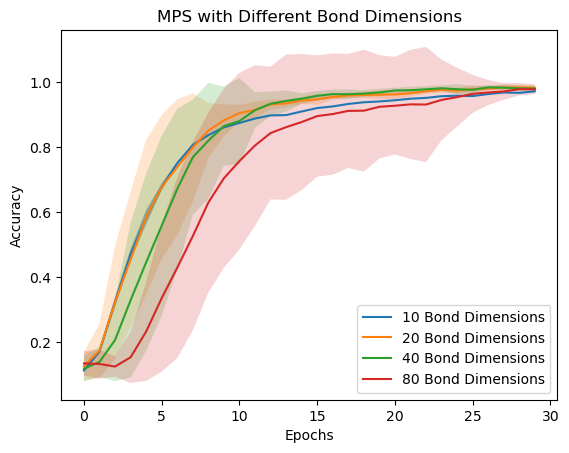
\includegraphics[width=0.8\textwidth]{images/2023-04-21-18-13-34.png}
    \label{fig:MPS}
\end{figure}

\begin{figure}[H]
    \centering
    \caption{}
    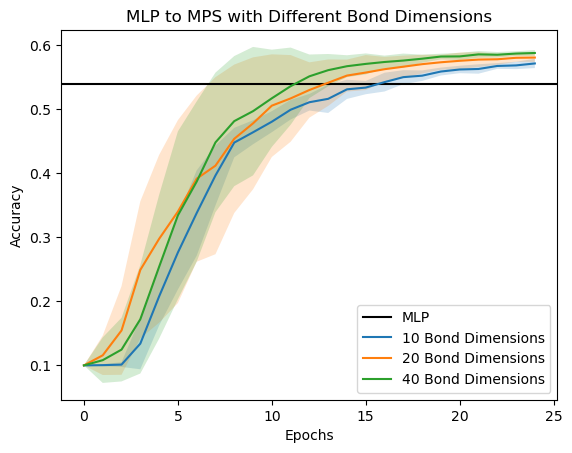
\includegraphics[width=0.8\textwidth]{images/images/2023-04-21-18-13-34.png.png}
    \label{fig:MLP_to_MPS}
\end{figure}

\begin{figure}[H]
    \centering
    \caption{}
    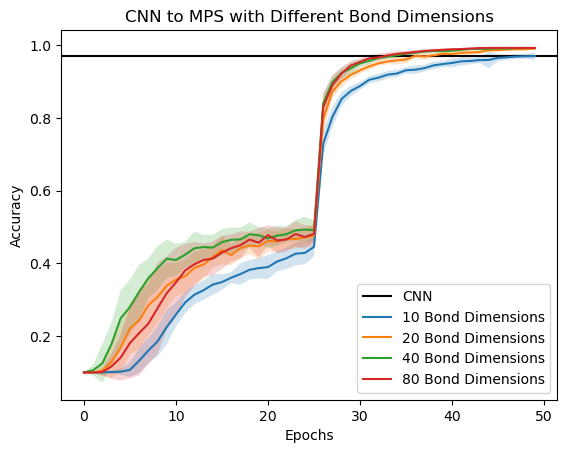
\includegraphics[width=0.8\textwidth]{images/2023-04-21-18-13-15.png}
    \label{fig:CNN_to_MPS}
\end{figure}

\section{Analysis}

\subsection{Bad Teacher : MLP to MPS}
\begin{figure}[hbt!]
    \centering
    \caption{Illustration of the role of bias and variance in the divergence between the model and the goal function.}
    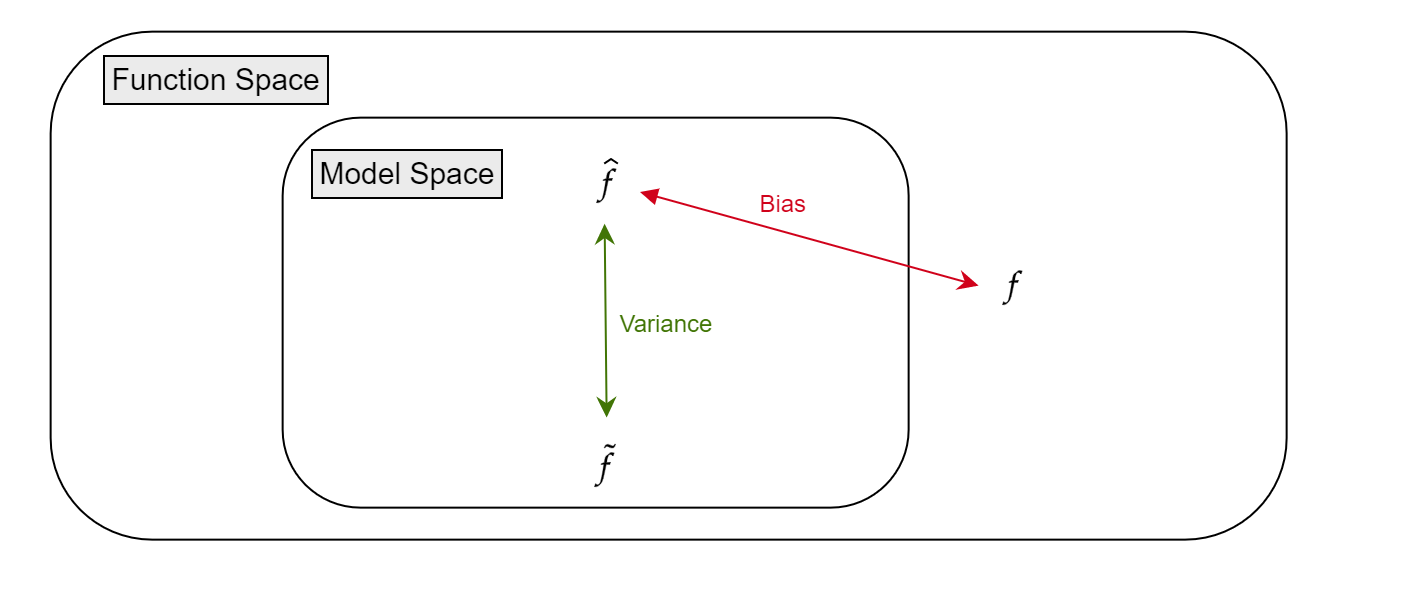
\includegraphics[width=0.8\textwidth]{images/2023-04-21-16-47-59.png}
    \floatfoot{Here, $f$ represents the goal function (the function we want to learn), $\hat{f}$ is the closest function to $f$ that our model can express and $\tilde{f}$ represents the function we can expect to obtain during training.}
    \label{fig:function_space}
\end{figure}

As you can see in Table \ref{tab:main}, the MPS, for bond dimensions 20 and 40,  generalises better on unseen test data than its own teacher. This is strange, because it has only seen the labels given by the bad teacher during training. One explanation for this is that student model is more biased towards the goal function $f$\footnote{The goal function is the function that our model is trying to learn.} than the MLP. Figure \ref{fig:function_space} might help us visualise this. In this figure, we can see that the distance from the learned function $\tilde{f}$ and the goal function $f$ is caused by a combination of variance and bias. Usually, the variance is caused by the stochasticity of the examples present in the training set {\bf and} the hyperparameters of the model. However, in our experiments, there was no variation in the training examples. All the models were trained on the same $2000$ handwritten digits. Thus, there was no disavantage to the teacher with regards to the examples contained in the training set. This means that the only source of variance was in the hyperparameters of the models. An example is the initial weights of the MPS network. We'd like to be able to conclude that the real cause of the slightly better accuracy from the student has more to do with the bias of the models. However, to confirm that there is less of a bias in the our MPS architecture than in the MLP, an additionnal experiment would be required. In this experiment, we would train $30$ bad teachers with our MLP architecture. Then, we would distill the knowledge of each of these bad teachers in the 20 MPS students, for a total of $600$ students trained. Then, if the the student performed better on average then their teachers, we could conclude that real cause of better accuracy from the student is because the MPS architecture is more biased towards the MNIST distribution than the MLP architecture we used for te teacher. \\ Another interesting aspect is the reduction of variance as we get past the $15$th epoch. If you look at Figure \ref{fig:MPS}, you can see that when the MPS is on its own, the reduction in the standard deviation of its accuracy happens later, at epoch 22.


\subsection{Good Teacher : CNN to MPS}
As you can see, from Table \ref{tab:main}, with the help of the good teacher, the MPS manages to perform better on average then when it learns on its own. Amazingly, this is true for every bond dimension in our experiments (10, 20, 40 and 80). However, this finding is, as of now, purely of theoretical use. This is due to the fact that the simple CNN we trained, which performs better than the MPS at every bond dimension, has way less parameters then the MPS. The CNN model has 93130 parameters, while the MPS with the lowest bond dimension we trained (10) had 158000 parameters.\\

As mentionned in the methodology, we used Gaussian noise on the first 25 epochs of the training. In Figure \ref{fig:CNN_to_MPS}, you can see the spike of accuracy when we stop adding Gaussian noise from epoch 26 onward. This might make you wonder if it would be better to not have Gaussian noise at all. Without showing you additionnal data, we can tell you that it is not the case. The Gaussian noise does help. Additionnaly, the order was really important. When applying the Gaussian noise after the initial training, the accuracy tended to drop instead of going up. You can also see that the standard deviation is much higher in the Gaussian epochs.



\subsection{Why did Backpropagation Fail to Train the DoubleMPS?}
Why did backpropagation fail so miserably to update the weights of our Double-MPS during training? Our leading hypothesis has to do with the exploding and vanishing gradient problems\cite{pascanu2013difficulty}. It could be due to the fact that with the the derivatives of the monomials produced by the DoubleMPS are still exponentials. If the values of the terms are $<1$, then their gradient could also get close to zero. If the values of the terms are too big, the gradient might explode. We would like to reiterate that these are merely hypotheses. \\

We would also like to mention that while we will not show results explicitely here, we use Layer-Based Knowledge distillation in order to train the DoubleMPS. The sudents trained always got close to the accuracy of their teacher, but never surpassed it.


\subsection{Further Exploration}
We think that using Tensor Networks for machine learning is a very interesting endeavour. However, we believe that some attachments to current practices are holding back interesting explorations. An example would be in the way that the inputs are placed in the network. In our implementation, the inputs were separated from the core MPS structure of the network. They were in their own little private external tensors and connected to MPS structure via indices. We think one way forward is to get rid of this hard separation, and introduce techniques to make the inputs part of the inner tensors of the network. Another would be to apply simple scalar non-linear transformations at every contraction, like a filter on the edges. \\


As structured data grows in complexity, we tend to flatten it and hope that the models learn the useful spacial relashionships between features on their own. Tensor Networks could provide a way to let the data in its arbitrary shape, therefore keeping crucial information underlying the connections between different feature proximities. This would hopefully lead to models more biased towards real world distributions.



\printbibliography
\end{document}




































Person 1: *waiving vigorously
    HELLO CAN YOU SEE ME!
    HEYYY! 

Person 2:
    For the last time, they can't see you... 
    YOU'\mathbb{R}E OUTSIDE THE DOCUMENT DELIMITE\mathbb{R}S!

Person 1: 
    I feel so alone... 

Person 2: 
    Bro I'm here... not need to worry $:)$